\section{Mössbauer Spectroscopy}

\frame[plain]{\tableofcontents[currentsection]}

\subsection{Experimental Setup}
	\begin{frame}
		\frametitle{Mössbauer spectrometer}
		
		\begin{block}{Construction}
			\begin{itemize}
				\item \textbf{Mössbauer Drive:} moving part which generates the Doppler effect
				\item \textbf{Collimator:} filters out non-parallel $\gamma$-rays
				\item \textbf{Detector}
			\end{itemize}
		\end{block}
		
		\begin{figure}
			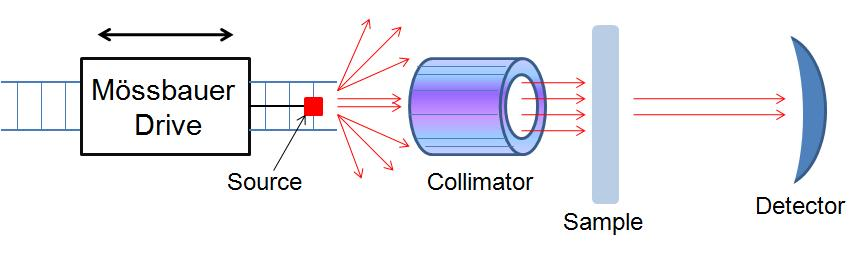
\includegraphics[width=6cm]{images/spectrometer.jpg}
			\credit{Wikipedia \cite{wiki:spectrometer}}
			\caption{Schematic view of Mössbauer spectrometer}
		\end{figure}
	\end{frame}

\subsection{Mössbauer Spectrum}
	\begin{frame}
		\frametitle{Mössbauer spectrum}
		\begin{figure}
			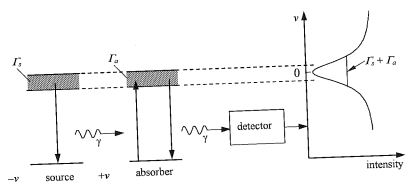
\includegraphics[width=8cm]{images/moessbauer-spectrum-measurement.jpg}
			\credit{Yi-Long Chen: Mössbauer Effect \cite{longyang07}}
			\caption{Measuring a Mössbauer spectrum}
		\end{figure}
		\begin{itemize}
			\item minimum linewidth $\Gamma_s+\Gamma_a$
			\item energy axis labelled using $v_x$ (source velocity in $mm s^{-1}$)
			\item energy value obtained by multiplying $v_x$ with $E_{\gamma}/c$ (i.e. $\ce{^{57}Fe}$: $\unit[4.8075 x 10^{-8}]{eV \thinspace mm^{-1} \thinspace s}$)
		\end{itemize}
	\end{frame}

\subsection{Hyperfine Interactions}
	\begin{frame}
		\frametitle{Hyperfine interactions}
		\begin{block}{Definition}
			Interactions between nucleus and electromagnetic fields produced by surrounding electrons, atoms or ions. They are very weak interactions.
		\end{block}
	
		\begin{block}{Types}
			\begin{itemize}
				\item \textbf{Isomer shift $\delta$:} electric monopole interaction
				\item \textbf{Quadrupole splitting:} electric quadrupole interaction
				\item \textbf{Zeeman splitting:} magnetic dipole interaction
			\end{itemize}
		\end{block}
	\end{frame}

\subsubsection{Isomer Shift}
	

	\begin{frame}
		\frametitle{Isomer Shift}
		
		\fontsize{10pt}{11pt}
		\begin{columns}
			\begin{column}{0.49\textwidth}
				\begin{block}{Definition}
					\begin{equation*}
					\delta E = \frac{2 \pi}{3} z e^2 | \psi(0) |^2 \langle r^2 \rangle
					\end{equation*}
					Nuclear energy levels shift $\delta E$
				\end{block}
			\end{column}
		
			\begin{column}{0.49\textwidth}
				Energy of emitted $\gamma$-ray:
				\begin{equation*}
					E_s=E_0+\delta E_s^e-\delta E_s^g
				\end{equation*}
				Condition for resonant recoilless absorption:
				\begin{equation*}
					E_a=E_0+\delta E_a^e-\delta E_a^g
				\end{equation*}
			\end{column}
		\end{columns}

		\begin{columns}
			\begin{column}{0.49\textwidth}
				\centering
				\begin{figure}
					\centering
					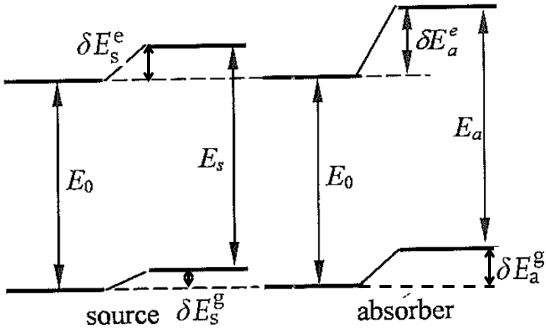
\includegraphics[width=4cm]{images/isomer-shift.jpg}
					\credit{Yi-Long Chen: Mössbauer Effect \cite{longyang07}}
					\caption{Shift of nuclear energy levels due to electric monopole interaction}
				\end{figure}
			\end{column}
			
			\begin{column}{0.49\textwidth}
				\begin{figure}
					\centering
					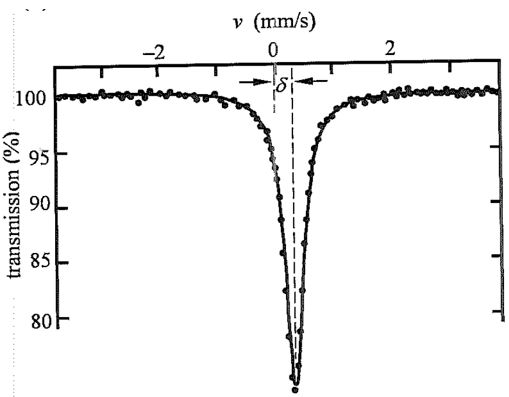
\includegraphics[width=4cm]{images/isomer-shift-spectrum.jpg}
					\credit{Yi-Long Chen: Mössbauer Effect \cite{longyang07}}
					\caption{Typical Mössbauer spectrum in the presence of an isomer shift}
				\end{figure}
			\end{column}
		\end{columns}
	\end{frame}

	\begin{frame}
		\frametitle{Isomer Shift}
		\centering
		\begin{block}{Provides information on}
			\begin{itemize}
				\item electronic structure
				\begin{enumerate}
					\item inner \textbf{s} electrons of the Mössbauer atom
					\item valence electrons in outer shells
					\item valence electrons of ligands
				\end{enumerate}
				\item type of chemical bond (covalent, metallic etc.)
				\item oxidation state
				\item spin state
				\item electronegativity of the ligands
				\item coordination number
			\end{itemize}
		\end{block}
	\end{frame}

	\begin{frame}
		\frametitle{Isomer Shift Calibration}
		Isomer shift $\delta$ is measured with respect to that of a reference absorber (source and absorber in different chemical environments):
		\begin{equation*}
			\delta=\delta_0-\delta_{ref}
		\end{equation*}
		
		\begin{description}
			\item[$\delta_0$] measured isomer shift
			\item[$\delta_{ref}$] isomer shift of reference absorber
		\end{description}
		
		\begin{figure}
			\centering
			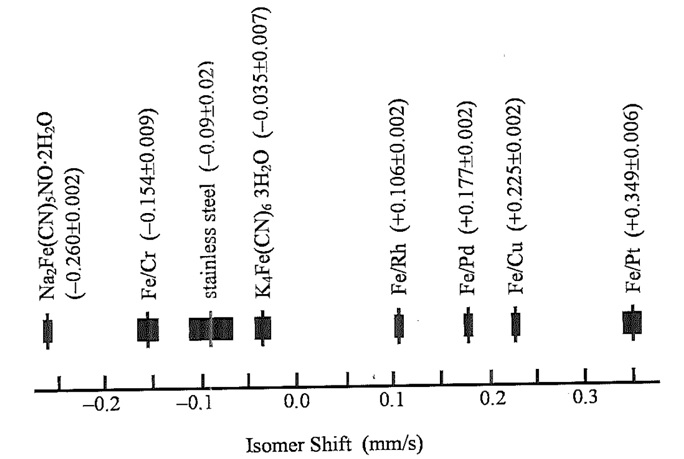
\includegraphics[width=6cm]{images/isomer-shift-calibration.jpg}
			\credit{Yi-Long Chen: Mössbauer Effect \cite{longyang07}}
			\caption{Isomer shifts of several reference absorbers}
		\end{figure}
	\end{frame}

\subsubsection{Quadrupole Splitting}

	\begin{frame}
		\frametitle{Quadrupole Splitting}
		\begin{block}{Why it happens?}
			\begin{enumerate}
				\item nucleus with an electric quadrupole moment experiences non-uniform electric field (electric field gradient, EFG)
				\item nuclear charge distribution has non-spherical symmetry if nucleus has spin quantum number \textbf{$I > 1/2$} and non-zero electric quadrupole moment
			\end{enumerate}
		
			\begin{figure}
				\centering
				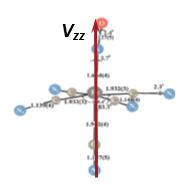
\includegraphics[width=3cm]{images/absorber-crystal-structure.png}
				\credit{V. Rusanov et al (2003) \cite{rusanov03}}
			\end{figure}
		\end{block}
	\end{frame}

	\begin{frame}
		\frametitle{Quadrupole Splitting}
		$V_{zz}$ is the electric field gradient due to total electron density plus all nuclear charges. Separation between the lines:
		\begin{equation*}
			\Delta E_Q=\frac{e Q V_{zz}}{2} \left( 1 + \frac{\eta^2}{3} \right)^{1/2}
		\end{equation*}
		
		\vspace{-0.6cm}
		\begin{columns}
			\begin{column}{0.49\textwidth}
				\begin{figure}
					\centering
					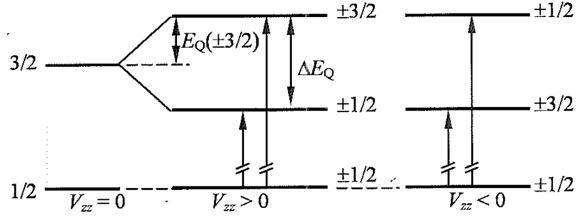
\includegraphics[width=6cm]{images/quadrupole-splitting.jpg}
					\credit{Yi-Long Chen: Mössbauer Effect \cite{longyang07}}
					\caption{Split $\ce{^{57}Fe}$ energy levels by quadrupole interaction}
				\end{figure}
			\end{column}
			\begin{column}{0.49\textwidth}
				\begin{figure}
					\centering
					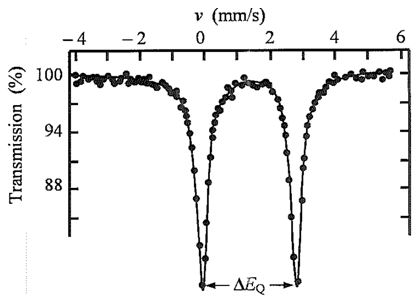
\includegraphics[width=5cm]{images/quadrupole-splitting-spectrum.jpg}
					\credit{Yi-Long Chen: Mössbauer Effect \cite{longyang07}}
					\caption{Quadrupole splitting Mössbauer spectrum}
				\end{figure}
			\end{column}
		\end{columns}
	\end{frame}

	\begin{frame}
		\frametitle{Zeeman Splitting}
		\begin{block}{Definition}
			The nuclear magnetic moment $\mu$ and the magnetic field $\vec{B}$ at the nucleus cause the magnetic hyperfine interaction.
		\end{block}
		\begin{block}{Details}
			\begin{enumerate}
				\item magnetic field is produced by surrounding electrons/ions
				\item degeneracy of $\vec{l}$ level is lifted
				\item level is split into $(2l+1)$ sublevels (Zeeman Splitting)
			\end{enumerate}
		\end{block}
	\end{frame}

\subsubsection{Zeeman Splitting}

	\begin{frame}
		\frametitle{Zeeman Splitting}
		
		\begin{columns}
			\begin{column}{0.49\textwidth}
				\begin{figure}
					\centering
					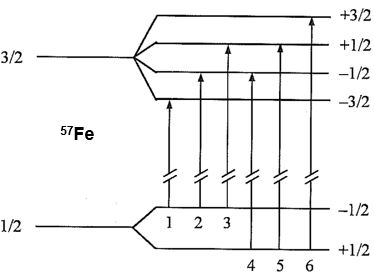
\includegraphics[width=4cm]{images/zeeman-splitting.jpg}
					\credit{Yi-Long Chen: Mössbauer Effect \cite{longyang07}}
					\caption{Magnetic splittings of the $\ce{^{57}Fe}$ nuclear energy levels}
				\end{figure}
			\end{column}
		
			\begin{column}{0.49\textwidth}
				\begin{figure}
					\centering
					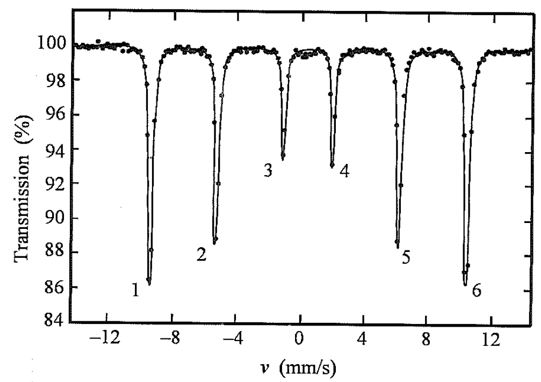
\includegraphics[width=5cm]{images/zeeman-spectrum.jpg}
					\credit{Yi-Long Chen: Mössbauer Effect \cite{longyang07}}
					\caption{Mössbauer spectrum of $\ce{FeF_3}$ with a sextet due to magnetic}
				\end{figure}
			\end{column}
		\end{columns}
	
		\begin{itemize}
			\item M1-magnetic dipole $\gamma$ transition in $^{57}\ce{Fe}$
			\item selection rule $\Delta m=\pm 1,0$
			\item 6 allowed sublevel transitions
		\end{itemize}
	\end{frame}

\subsection{Applications}

	\begin{frame}
		\frametitle{Applications}
		Mars Exploration Rover ''Spirit'' and ''Opportunity'' Missions studying iron-containing minerals
		\begin{figure}[t!]
			\begin{subfigure}
				\centering
				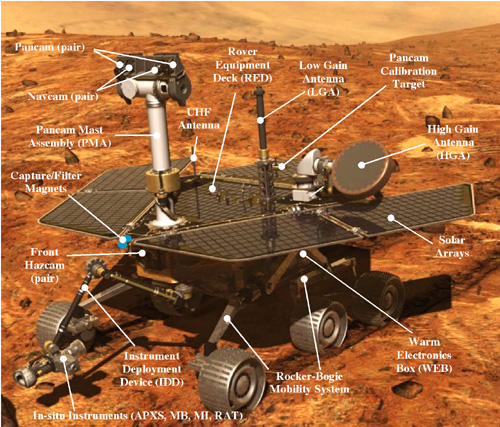
\includegraphics[width=5cm]{images/mars-rover-2.jpg}
			\end{subfigure}
			~
			\begin{subfigure}
				\centering
				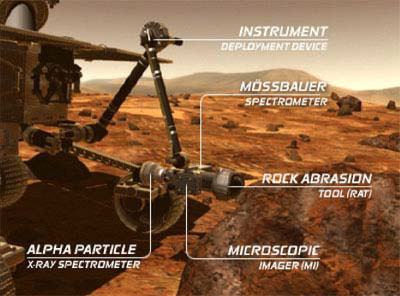
\includegraphics[width=5cm]{images/mars-rover.jpg}
			\end{subfigure}
			\credit{exploratorium.edu, thetimenow.com/astronomy \cite{web:mossbauer4} \cite{web:mossbauer3}}
			\caption{Mars Exploration Rover}
		\end{figure}
	\end{frame}

	\begin{frame}
		\frametitle{Applications}
		Mars Exploration Rover ''Spirit'' and ''Opportunity'' Missions studying iron-containing minerals
		\begin{figure}
			\centering
			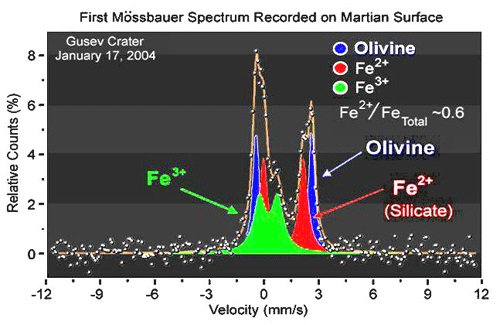
\includegraphics[width=7cm]{images/mars-spectrum.jpg}
			\credit{mossbauer.info \cite{web:mossbauer5}}
		\end{figure}
	\end{frame}